\documentclass[grid,avery5371]{flashcards}
\usepackage{amssymb}
\usepackage[utf8]{inputenc}
\usepackage[T1]{fontenc}
\usepackage{verse}
\usepackage[version=3]{mhchem}
\usepackage{graphicx}
\settowidth{\versewidth}{It lies behind stars and under hills,}
\addtolength{\versewidth}{2em}
\usepackage{pgfplots}
\geometry{headheight=12pt}
\usepackage{fancyhdr}
\pagestyle{fancy}
\fancyhf{}
\renewcommand{\headrulewidth}{0pt}


\title{Conversion flashcards}
\author{Sam Robbins}

\cardbackstyle[\large]{plain}
\cardfrontstyle[\large]{headings}
%\cardbackstyle[\large]{headings}

\begin{document}

\begin{flashcard}[]{\Huge{$e^x$}}
\begin{tikzpicture}[scale=0.8]
\begin{axis}[ymin=0,ticks=none]
\addplot[color=red,domain=-2:2]{exp(x)};
\draw[ultra thin] (axis cs:0,\pgfkeysvalueof{/pgfplots/ymin}) -- (axis cs:0,\pgfkeysvalueof{/pgfplots/ymax});
\draw[ultra thin] (axis cs:\pgfkeysvalueof{/pgfplots/xmin},0) -- (axis cs:\pgfkeysvalueof{/pgfplots/xmax},0);

\end{axis}
\end{tikzpicture}
\end{flashcard}

\begin{flashcard}[]{\Huge{$e^{-x}$}}
\begin{tikzpicture}[scale=0.8]
\begin{axis}[ymin=0,ticks=none]
\addplot[color=red, domain=-2:2]{1/exp(x)};
\draw[ultra thin] (axis cs:0,\pgfkeysvalueof{/pgfplots/ymin}) -- (axis cs:0,\pgfkeysvalueof{/pgfplots/ymax});
\draw[ultra thin] (axis cs:\pgfkeysvalueof{/pgfplots/xmin},0) -- (axis cs:\pgfkeysvalueof{/pgfplots/xmax},0);

\end{axis}
\end{tikzpicture}
\end{flashcard}

\begin{flashcard}[]{\Huge{\textcolor{red}{$e^x$}\\$e^{2x}$}}
\begin{tikzpicture}[scale=0.8]
\begin{axis}[ymin=0,ticks=none]
\addplot[color=black,domain=-1:1, ]{e^(2*x)};
\addplot[color=red,domain=-2:2, ]{exp(x)};
\draw[ultra thin] (axis cs:0,\pgfkeysvalueof{/pgfplots/ymin}) -- (axis cs:0,\pgfkeysvalueof{/pgfplots/ymax});
\draw[ultra thin] (axis cs:\pgfkeysvalueof{/pgfplots/xmin},0) -- (axis cs:\pgfkeysvalueof{/pgfplots/xmax},0);

\end{axis}
\end{tikzpicture}
\end{flashcard}

\begin{flashcard}[]{\Huge{\textcolor{red}{$e^{-x}$}\\$10e^{-x}$}}
\begin{tikzpicture}[scale=0.8]
\begin{axis}[ymin=0,ticks=none]
\addplot[color=black,domain=-1:1]{(10*(e^(-x)))};
\addplot[color=red,domain=-1:1]{1/e^(x)};
\draw[ultra thin] (axis cs:0,\pgfkeysvalueof{/pgfplots/ymin}) -- (axis cs:0,\pgfkeysvalueof{/pgfplots/ymax});
\draw[ultra thin] (axis cs:\pgfkeysvalueof{/pgfplots/xmin},0) -- (axis cs:\pgfkeysvalueof{/pgfplots/xmax},0);

\end{axis}
\end{tikzpicture}
\end{flashcard}

\begin{flashcard}[]{\Huge{\textcolor{red}{$e^{x}$}\\$\ln x$}}
\begin{tikzpicture}[scale=0.8]
\begin{axis}[ticks=none]
\addplot[color=black,domain=0:4, ]{ln(x)};
\addplot[color=red,domain=-2:2, ]{exp(x)};
\draw[ultra thin] (axis cs:0,\pgfkeysvalueof{/pgfplots/ymin}) -- (axis cs:0,\pgfkeysvalueof{/pgfplots/ymax});
\draw[ultra thin] (axis cs:\pgfkeysvalueof{/pgfplots/xmin},0) -- (axis cs:\pgfkeysvalueof{/pgfplots/xmax},0);

\end{axis}
\end{tikzpicture}

\end{flashcard}

\begin{flashcard}[$y=|x|$]{

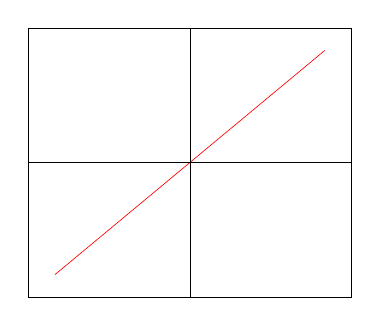
\begin{tikzpicture}[scale=0.6]
\begin{axis}[ticks=none]
\addplot[color=red,domain=-4:4, ]{x};
\draw[ultra thin] (axis cs:0,\pgfkeysvalueof{/pgfplots/ymin}) -- (axis cs:0,\pgfkeysvalueof{/pgfplots/ymax});
\draw[ultra thin] (axis cs:\pgfkeysvalueof{/pgfplots/xmin},0) -- (axis cs:\pgfkeysvalueof{/pgfplots/xmax},0);
\end{axis}
\end{tikzpicture}\\
$y=x$}
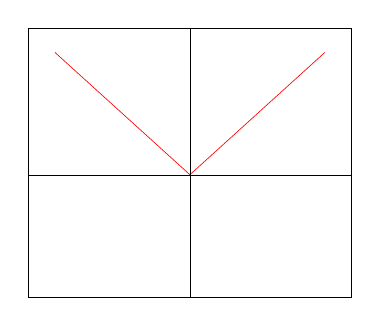
\begin{tikzpicture}[scale=0.6]
\begin{axis}[ymin=-4,ticks=none]
\addplot[color=red,domain=-4:4, ]{abs(x)};
\draw[ultra thin] (axis cs:0,\pgfkeysvalueof{/pgfplots/ymin}) -- (axis cs:0,\pgfkeysvalueof{/pgfplots/ymax});
\draw[ultra thin] (axis cs:\pgfkeysvalueof{/pgfplots/xmin},0) -- (axis cs:\pgfkeysvalueof{/pgfplots/xmax},0);
\end{axis}
\end{tikzpicture}\\
$y=|x|$
\end{flashcard}

\begin{flashcard}[$y=|3x-2|$]{
\begin{tikzpicture}[scale=0.6]
\begin{axis}[ymin=-10,ymax=10,ticks=none]
\addplot[color=red,domain=-2:3, ]{3*x-2};
\draw[ultra thin] (axis cs:0,\pgfkeysvalueof{/pgfplots/ymin}) -- (axis cs:0,\pgfkeysvalueof{/pgfplots/ymax});
\draw[ultra thin] (axis cs:\pgfkeysvalueof{/pgfplots/xmin},0) -- (axis cs:\pgfkeysvalueof{/pgfplots/xmax},0);
\end{axis}
\end{tikzpicture}\\
$y=3x-2$}
\begin{tikzpicture}[scale=0.6]
\begin{axis}[ymin=-10,ymax=10,ticks=none]
\addplot[color=red,domain=-2:3,samples=300 ]{abs(3*x-2)};
\draw[ultra thin] (axis cs:0,\pgfkeysvalueof{/pgfplots/ymin}) -- (axis cs:0,\pgfkeysvalueof{/pgfplots/ymax});
\draw[ultra thin] (axis cs:\pgfkeysvalueof{/pgfplots/xmin},0) -- (axis cs:\pgfkeysvalueof{/pgfplots/xmax},0);
\end{axis}
\end{tikzpicture}\\
$y=|3x-2|$
\end{flashcard}

\begin{flashcard}[$y=|x^2-3x-10|$]{
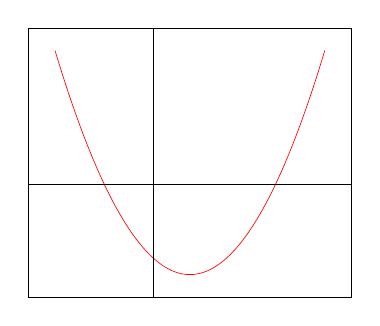
\begin{tikzpicture}[scale=0.6]
\begin{axis}[ticks=none]
\addplot[color=red,domain=-4:7,samples=100 ]{x^2-3*x-10};
\draw[ultra thin] (axis cs:0,\pgfkeysvalueof{/pgfplots/ymin}) -- (axis cs:0,\pgfkeysvalueof{/pgfplots/ymax});
\draw[ultra thin] (axis cs:\pgfkeysvalueof{/pgfplots/xmin},0) -- (axis cs:\pgfkeysvalueof{/pgfplots/xmax},0);
\end{axis}
\end{tikzpicture}\\
$y=x^2-3x-10$}

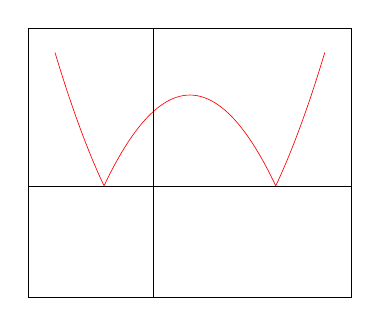
\begin{tikzpicture}[scale=0.6]
\begin{axis}[ymin=-15,ticks=none]
\addplot[color=red,domain=-4:7,samples=500 ]{abs(x^2-3*x-10)};
\draw[ultra thin] (axis cs:0,\pgfkeysvalueof{/pgfplots/ymin}) -- (axis cs:0,\pgfkeysvalueof{/pgfplots/ymax});
\draw[ultra thin] (axis cs:\pgfkeysvalueof{/pgfplots/xmin},0) -- (axis cs:\pgfkeysvalueof{/pgfplots/xmax},0);
\end{axis}
\end{tikzpicture}\\
$y=|x^2-3x-10|$

\end{flashcard}

\begin{flashcard}[$y=|\sin(x)|$]{
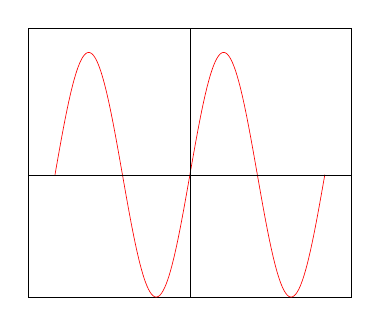
\begin{tikzpicture}[scale=0.6]
\begin{axis}[ymin=-1,ticks=none]
\addplot[color=red,domain=-360:360,samples=500 ]{sin(x)};
\draw[ultra thin] (axis cs:0,\pgfkeysvalueof{/pgfplots/ymin}) -- (axis cs:0,\pgfkeysvalueof{/pgfplots/ymax});
\draw[ultra thin] (axis cs:\pgfkeysvalueof{/pgfplots/xmin},0) -- (axis cs:\pgfkeysvalueof{/pgfplots/xmax},0);
\end{axis}
\end{tikzpicture}\\
$y=\sin(x)$}
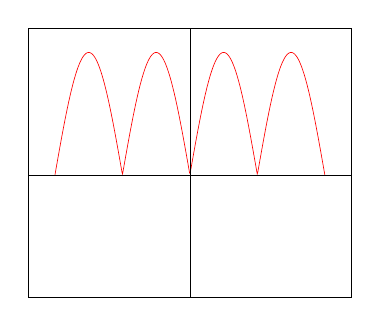
\begin{tikzpicture}[scale=0.6]
\begin{axis}[ymin=-1,ticks=none]
\addplot[color=red,domain=-360:360,samples=500 ]{abs(sin(x))};
\draw[ultra thin] (axis cs:0,\pgfkeysvalueof{/pgfplots/ymin}) -- (axis cs:0,\pgfkeysvalueof{/pgfplots/ymax});
\draw[ultra thin] (axis cs:\pgfkeysvalueof{/pgfplots/xmin},0) -- (axis cs:\pgfkeysvalueof{/pgfplots/xmax},0);
\end{axis}
\end{tikzpicture}\\
$y=|\sin(x)|$      
\end{flashcard}

\begin{flashcard}[$y=4|x|-|x|^3$]{
\begin{tikzpicture}[scale=0.6]
\begin{axis}[ymin=-4,xmin=-4,xmax=4,ticks=none]
\addplot[color=red,domain=0:4,samples=500 ]{4*x-x^3};
\draw[ultra thin] (axis cs:0,\pgfkeysvalueof{/pgfplots/ymin}) -- (axis cs:0,\pgfkeysvalueof{/pgfplots/ymax});
\draw[ultra thin] (axis cs:\pgfkeysvalueof{/pgfplots/xmin},0) -- (axis cs:\pgfkeysvalueof{/pgfplots/xmax},0);
\end{axis}
\end{tikzpicture}\\
$y=4x-x^3,x\geqslant0$

}
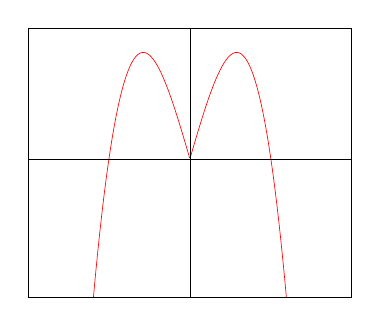
\begin{tikzpicture}[scale=0.6]
\begin{axis}[ymin=-4,xmax=4,xmin=-4,ticks=none]
\addplot[color=red,domain=-4:4,samples=500 ]{4*abs(x)-(abs(x))^3};
\draw[ultra thin] (axis cs:0,\pgfkeysvalueof{/pgfplots/ymin}) -- (axis cs:0,\pgfkeysvalueof{/pgfplots/ymax});
\draw[ultra thin] (axis cs:\pgfkeysvalueof{/pgfplots/xmin},0) -- (axis cs:\pgfkeysvalueof{/pgfplots/xmax},0);
\end{axis}
\end{tikzpicture}\\
$y=4|x|-|x|^3$
\end{flashcard}

\begin{flashcard}[]{\Huge{f(x+a)}}
\Huge{Horizontal translation of \textbf{-a}}
\end{flashcard}

\begin{flashcard}[]{\Huge{f(x)+a}}
\Huge{Vertical translation of \textbf{+a}}
\end{flashcard}

\begin{flashcard}[]{\Huge{f(ax)}}
\Huge{Horizontal stretch of scale factor $\mathbf{\frac{1}{a}}$}
\end{flashcard}

\begin{flashcard}[]{\Huge{f(-x)}}
\Huge{Reflection in the\\ \textbf{y axis}}
\end{flashcard}

\begin{flashcard}[]{\Huge{af(x)}}
\Huge{Vertical stretch of scale factor \textbf{a}}
\end{flashcard}

\begin{flashcard}[]{\Huge{-f(x)}}
\Huge{Reflection in the\\ \textbf{x axis}}
\end{flashcard}

\begin{flashcard}[]{\Huge{$\sec\theta$}}
\Huge{$\dfrac{1}{\cos\theta}$}
\end{flashcard}

\begin{flashcard}[]{\Huge{$\csc\theta$}}
\Huge{$\dfrac{1}{\sin\theta}$}
\end{flashcard}

\begin{flashcard}[]{\Huge{$\cot\theta$}}
\Huge{$\dfrac{1}{\tan\theta}=\dfrac{\cos\theta}{\sin\theta}$}
\end{flashcard}

\begin{flashcard}[]{\Huge{Graph of $\sec\theta$}}
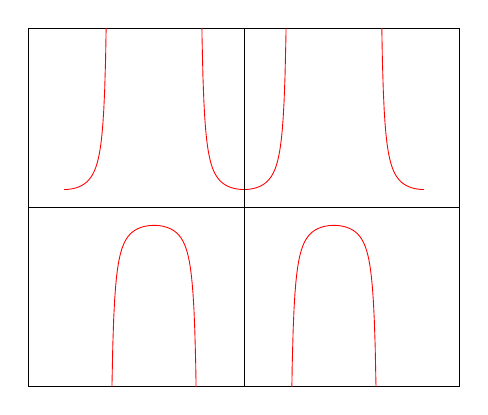
\begin{tikzpicture}[scale=0.8]
\begin{axis}[ymax=10,ymin=-10,ticks=none]
\addplot[color=red,domain=-360:360,samples=400,restrict y to domain=-15:15]
{sec(x)};
\draw[ultra thin] (axis cs:0,\pgfkeysvalueof{/pgfplots/ymin}) -- (axis 
cs:0,\pgfkeysvalueof{/pgfplots/ymax});
\draw[ultra thin] (axis cs:\pgfkeysvalueof{/pgfplots/xmin},0) -- (axis 
cs:\pgfkeysvalueof{/pgfplots/xmax},0);
\end{axis}
\end{tikzpicture}
\end{flashcard}

\begin{flashcard}[]{\Huge{Graph of $\csc\theta$}}
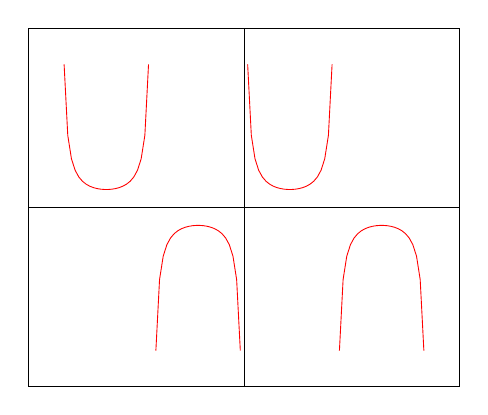
\begin{tikzpicture}[scale=0.8]
\begin{axis}[ymax=10,ymin=-10,ticks=none]
\addplot[color=red,domain=-360:360,samples=101,unbounded coords=jump]{cosec(x)};
\draw[ultra thin] (axis cs:0,\pgfkeysvalueof{/pgfplots/ymin}) -- (axis cs:0,\pgfkeysvalueof{/pgfplots/ymax});
\draw[ultra thin] (axis cs:\pgfkeysvalueof{/pgfplots/xmin},0) -- (axis cs:\pgfkeysvalueof{/pgfplots/xmax},0);
\end{axis}
\end{tikzpicture}
\end{flashcard}

\begin{flashcard}[]{\Huge{Graph of $\cot\theta$}}
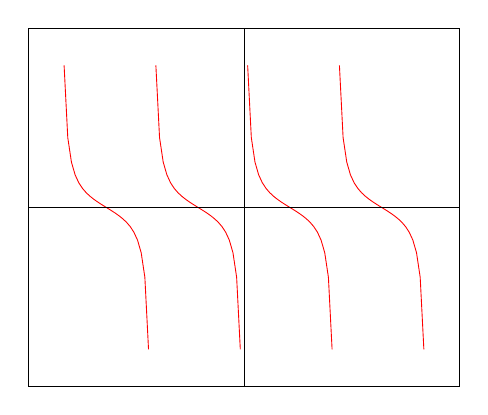
\begin{tikzpicture}[scale=0.8]
\begin{axis}[ymax=10,ymin=-10,ticks=none]
\addplot[color=red,domain=-360:360,samples=101,unbounded coords=jump]{cot(x)};
\draw[ultra thin] (axis cs:0,\pgfkeysvalueof{/pgfplots/ymin}) -- (axis cs:0,\pgfkeysvalueof{/pgfplots/ymax});
\draw[ultra thin] (axis cs:\pgfkeysvalueof{/pgfplots/xmin},0) -- (axis cs:\pgfkeysvalueof{/pgfplots/xmax},0);
\end{axis}
\end{tikzpicture}
\end{flashcard}

\begin{flashcard}[]{\Huge{$\sec^2\theta$}}
\Huge{$1+\tan^2\theta$}
\end{flashcard}

\begin{flashcard}[]{\Huge{$\csc^2\theta$}}
\Huge{$1+\cot^2\theta$}
\end{flashcard}

\begin{flashcard}[]{\Huge{Graph of $\arcsin\theta$}}
\begin{tikzpicture}[]
  \begin{axis}[domain = -1:1, samples = 100,ytick style={draw=none},xtick style={draw=none},scale=0.7]
    \addplot[color = red]  {asin(x)/180*pi};
      \end{axis}
\end{tikzpicture}
\end{flashcard}

\begin{flashcard}[]{\Huge{Graph of $\arccos\theta$}}
\begin{tikzpicture}[]
  \begin{axis}[domain = -1:1, samples = 100,ytick style={draw=none},xtick style={draw=none},scale=0.7]
    \addplot[color = red]  {acos(x)/180*pi};
      \end{axis}
\end{tikzpicture}
\end{flashcard}

\begin{flashcard}[]{\Huge{Graph of $\arctan\theta$}}
\begin{tikzpicture}[]
  \begin{axis}[domain = -1:1, samples = 100,ytick style={draw=none},xtick style={draw=none},scale=0.7]
    \addplot[color = red]  {atan(x)/180*pi};
      \end{axis}
\end{tikzpicture}
\end{flashcard}

\begin{flashcard}[]{\Huge{$y=[f(x)]^n$}}
\Huge{$\dfrac{dy}{dx}=n[f(x)]^{n-1}f'(x)$}
\end{flashcard}

\begin{flashcard}[]{\Huge{$y=f[g(x)]$}}
\Huge{$\dfrac{dy}{dx}=f'[g(x)]g'(x)$}
\end{flashcard}

\begin{flashcard}[]{\Huge{$y=uv$}}
\Huge{$\dfrac{dy}{dx}=u\dfrac{dv}{dx}+v\dfrac{du}{dx}$}
\end{flashcard}








\end{document}